% file: 2-9-sorting-selection/second-largest-roadmap.tex

\documentclass[tikz]{standalone}
\usetikzlibrary{positioning, backgrounds, fit}

\begin{document}
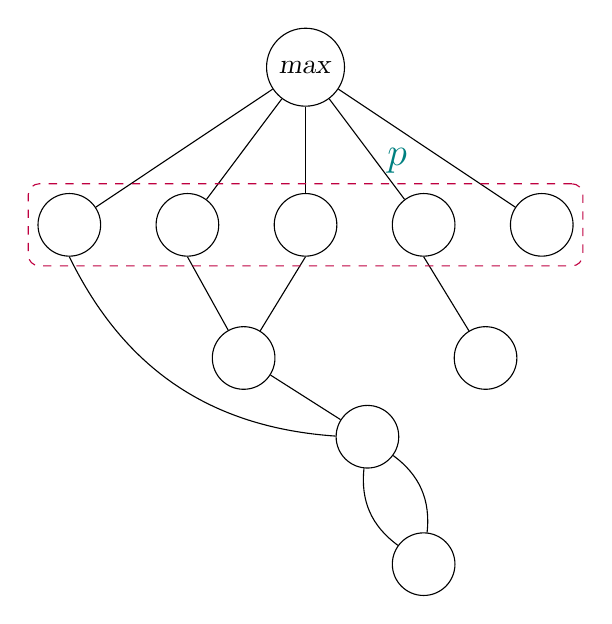
\begin{tikzpicture}[key/.style = {circle, draw, inner sep = 8pt}]
  \node (max) [circle, draw] {\textsl{max}};

  \foreach \i in {-2, ..., 2} {
    \node (\i) [key, below right = 1.5 cm and 1.5*\i cm of max.south, anchor = center] {};
    \draw[] (max) to (\i);
  }

  \node (A) [key, below left = 1.0cm and 0.5cm of 0.south] {};
  \draw (A) -- (0.south);
  \draw (A) -- (-1.south);

  \node (B) [key, below right = 1.0cm and 0.5cm of 1.south] {};
  \draw (B) -- (1.south);

  \node (C) [key, below right = 2.0cm and 0.5cm of 0.south] {};
  \node (D) [key, below = 3.5cm of 1.south] {};
  \draw[bend left] (C) to (D);
  \draw[bend left] (D) to (C);

  \draw (C) to (A);
  \draw[bend left] (C) to (-2.south);

  \begin{scope}{on background layer}
    \node () [rectangle, rounded corners, draw, purple, dashed, fit = (-2) (2), label = {[font = \Large, teal] 30 : $p$}] {};
  \end{scope}
\end{tikzpicture}
\end{document}
